\documentclass{article}
\usepackage{amsmath}
\usepackage{tikz}
\usetikzlibrary{matrix, arrows.meta}

\begin{document}

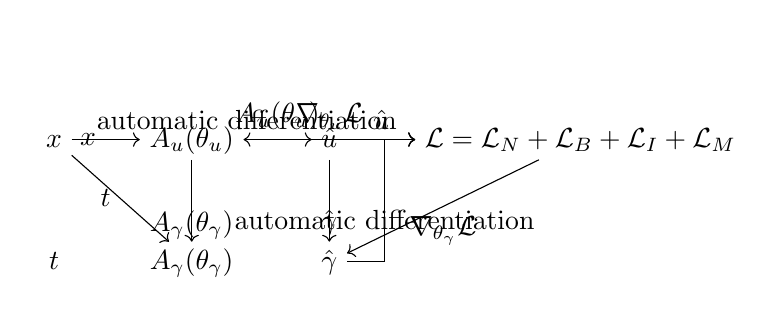
\begin{tikzpicture}[description/.style={fill=white,inner sep=2pt}]
    \matrix (m) [matrix of math nodes, row sep=3em, column sep=2.5em, text height=1.5ex, text depth=0.25ex]
    {
        & & & \\
        x & A_u(\theta_u) & \hat{u} & \mathcal{L} = \mathcal{L}_N + \mathcal{L}_B + \mathcal{L}_I + \mathcal{L}_M \\
        t & A_\gamma(\theta_\gamma) & \hat{\gamma} & \\
    };
    \path[->]
    (m-2-1) edge node[left] {$x$} (m-2-2)
            edge node[left] {$t$} (m-3-2)
    (m-2-2) edge node[above] {$A_u(\theta_u)$} (m-2-3)
            edge node[below] {$A_\gamma(\theta_\gamma)$} (m-3-2)
    (m-2-3) edge node[above] {$\hat{u}$} (m-2-4)
            edge node[below] {$\hat{\gamma}$} (m-3-3)
    (m-2-4) edge node[above] {$\nabla_{\theta_u}\mathcal{L}$} (m-2-2)
            edge node[below] {$\nabla_{\theta_\gamma}\mathcal{L}$} (m-3-3);
    \draw[->] (m-2-2) -- ++(0:.7cm) |- (m-2-4) node[pos=.25, above] {automatic differentiation};
    \draw[->] (m-3-3) -- ++(0:.7cm) |- (m-2-4) node[pos=.25, below] {automatic differentiation};
\end{tikzpicture}

\end{document}